%
% bio.tex — Éric Mugnier · biographie & coordonnées
% Compilation : latexmk -pdf bio.tex
%
\pdfminorversion=7
\documentclass[12pt,a4paper]{article}

\usepackage[utf8]{inputenc}
\usepackage[T1]{fontenc}
\usepackage{ebgaramond}
\usepackage[french]{babel}
\usepackage{microtype}
\usepackage{graphicx}
\usepackage{booktabs}
\usepackage{array}
\usepackage[left=30mm,right=25mm,top=28mm,bottom=25mm]{geometry}

\setlength{\parindent}{0pt}
\setlength{\parskip}{7pt}

\begin{document}
\pagestyle{empty}

% ─── Biographie ────────────────────────────────────────────────────────────────
\begin{tabular}{@{}p{3cm}p{11cm}@{}}
\toprule
\textsc{Biographie} & \\
\midrule
& Éric Mugnier a 65 ans ; \\
& habite la préfecture de l'un des départements les plus boisés de France, la Haute-Marne ; \\
& a été adopté tout petit via l'Assistance Publique par une mère seule de la moyenne bourgeoisie catholique locale ; \\
& n'a jamais eu d'activité professionnelle \og classique \fg{} : emploi, métier, profession, poste, travail, fonction, rien de tout cela ; \\
& a pu consacrer sa vie à la création, dans de nombreux arts : peinture, musique, chansons, et ici, écriture ; \\
& son auteur favori est Joris-Karl Huysmans. \\
\bottomrule
\end{tabular}

\bigskip

% ─── Coordonnées ───────────────────────────────────────────────────────────────
\begin{tabular}{@{}p{3cm}p{11cm}@{}}
\toprule
\textsc{Coordonnées} & \\
\midrule
& Éric Mugnier \\
& 33-11 rue Bouchardon \\
& 52000 Chaumont \\
& ericmugnier730@gmail.com \\
& 06 82 03 69 48 \\
\bottomrule
\end{tabular}

\bigskip\bigskip

% ─── Portrait ──────────────────────────────────────────────────────────────────
\begin{center}
  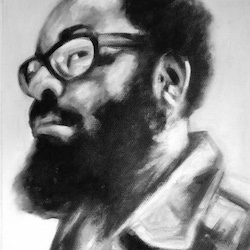
\includegraphics[width=0.5\linewidth]{images/Mugnier4.jpg}\\[4pt]
  \small Autoportrait, 2020
\end{center}

\end{document}
